%%%%%%%%%%%%%%%%%%%%%%%%%%%%%%%%%%%%%%%%%%%%%%%%%%%%%%
% A Beamer template for Ritsumeikan University       %
% Author: Ming-Hao Xu (Xu Minghao)                   %
% Date:   April 2022.                                %
% LPPL Licensed.                                     %
%%%%%%%%%%%%%%%%%%%%%%%%%%%%%%%%%%%%%%%%%%%%%%%%%%%%%%

\documentclass{beamer}
\usepackage{hyperref}

\usepackage[UTF8]{ctex}
\usepackage[T1]{fontenc}

% other packages
\usepackage{latexsym,amsmath,xcolor,multicol,booktabs,calligra}
\usepackage{graphicx,pstricks,listings,stackengine}
\usefonttheme[onlymath]{serif}

% dummy text; remove it when working on this template
\usepackage{lipsum}

\author{Ebola}
\title{高级字符串算法:字符串的后缀结构}
\institute{
    Institute of Mathematics, \\
    Zhejiang University.
}
\date{July, 2023}
\usepackage{Ritsumeikan}

% defs
\def\cmd#1{\texttt{\color{red}\footnotesize $\backslash$#1}}
\def\env#1{\texttt{\color{blue}\footnotesize #1}}
\definecolor{deepblue}{rgb}{0,0,0.5}
\definecolor{deepred}{rgb}{0.6,0,0}
\definecolor{deepgreen}{rgb}{0,0.5,0}
\definecolor{halfgray}{gray}{0.55}

\lstset{
    basicstyle=\ttfamily\tiny,
    keywordstyle=\bfseries\color{deepblue},
    emphstyle=\ttfamily\color{deepred},    % Custom highlighting style
    stringstyle=\color{deepgreen},
    numbers=left,
    numberstyle=\small\color{halfgray},
    rulesepcolor=\color{red!20!green!20!blue!20},
    frame=shadowbox,
}


\begin{document}

\begin{frame}
    \titlepage
\end{frame}

\begin{frame}
    \tableofcontents[sectionstyle=show,subsectionstyle=show/shaded/hide,subsubsectionstyle=show/shaded/hide]
\end{frame}

\section{后缀自动机}

\begin{frame}{模板题}
    \small
    给定一个只包含小写字母的字符串$S$,求$S$的所有出现次数不为$1$的子串的出现次数乘上该子串长度的最大值。$|S|\leq 10^6$
\end{frame}

\begin{frame}{什么是SAM}
    \small
    后缀自动机(SAM)是一种特殊的有限状态自动机(DFA),它符合以下性质:

    \begin{itemize}
        \item 转移图是有向无环图,且每个转移接受且只接受一个字符
        \item 接受且只接受$S$的所有后缀
        \item 在符合以上性质的基础上,节点数最少
    \end{itemize}
    
    如果只考虑前两条,其实只要把$S$的所有后缀插入字典树即可,节点数有$O(n^2)$个。
\end{frame}

\begin{frame}[fragile]{代码}
    \begin{minipage}{\linewidth}
    \begin{lstlisting}[language=c++]
        void insert(int c)
        {
            int p=lst,np=++tot;len[np]=len[p]+1;
            while(p&&!ch[p][c]) ch[p][c]=np,p=prt[p];
            if(!p) prt[np]=1;
            else
            {
                int q=ch[p][c];
                if(len[p]+1==len[q]) prt[np]=q;
                else
                {
                    int nq=++tot;len[nq]=len[p]+1;
                    memcpy(ch[nq],ch[q],sizeof(ch[nq]));
                    prt[nq]=prt[q];prt[q]=prt[np]=nq;
                    while(ch[p][c]==q) ch[p][c]=nq,p=prt[p];
                }
            }
            sz[np]=1;lst=np;
        }
    \end{lstlisting}
    \end{minipage}

    这是SAM的核心代码,很短。
\end{frame}

\begin{frame}{endpos等价类}
    \small
    我们首先提出endpos等价类这个概念。$endpos(P)$表示模式串$P$在$S$中所有出现的结束位置的集合,那么$endpos$相同的模式串就可以共用一个节点。例如串"aababc"中,"b"和"ab"的endpos都是$\{3,5\}$,说明他们总是一起出现,所以可以共用一个节点。我们把$endpos$相同的模式串组成的集合称为一个$endpos$ \textbf{等价类}。

    \pause \vspace{1em}
    显然,对于一个等价类内的两个模式串$P_1$和$P_2$,如果$|P_1|<|P_2|$,那么$P_1$一定是$P_2$的后缀,因此,在一个等价类中,一定存在一个\textbf{最长}的字符串$P$,等价类中的所有字符串都是$P$的后缀。

    \pause \vspace{1em}
    根据位于$P$ \textbf{前面的那一个字符}是什么,可以把原等价类划分为若干个等价类。例如在"aababc"中,我们已经知道"ab"出现了两次,但首次出现时前面的那一个字符是"a",再次出现时前面那个字符是"b",而"aab"与"bab"属于两个不同的等价类,因此我们可以把等价类$\{3,5\}$划分成$\{3\}$和$\{5\}$
\end{frame}

\begin{frame}{endpos等价类}
    \small
    我们可以认为,空串的$endpos$等价类是$\{1,...,n\}$,而所有等价类都是由此一步一步划分来的,形成一个树的结构,总节点数不会超过$2n-1$

    \begin{figure}[H]
        \centering
        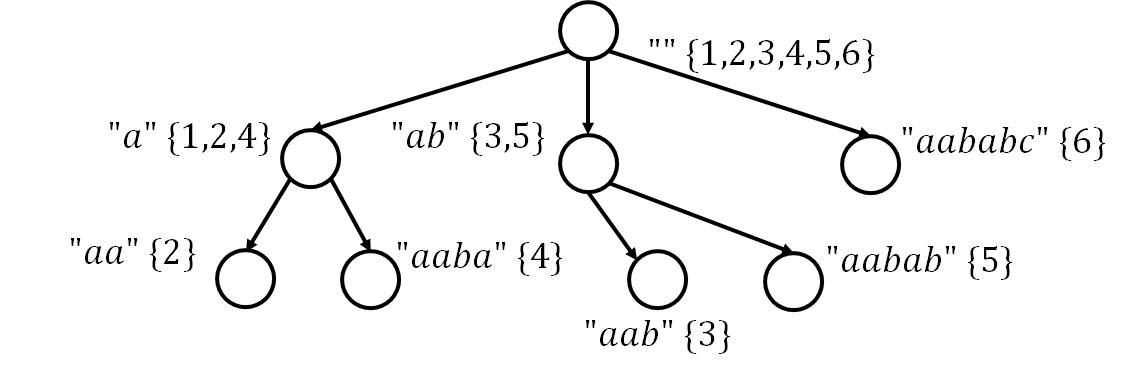
\includegraphics[width=0.7\textwidth]{pic/parent.png}
    \end{figure}

    这棵树就是parent树,他的节点和SAM的状态一一对应。注意,划分过程中可能会丢失元素,例如图中"a"第一个出现的位置前面没有字符,所以划分后会丢失一个元素,这一点在做dp的时候很关键。
\end{frame}

\begin{frame}{构造SAM}
    \small
采取动态构造的方法,一个一个地把字符加进去。考虑向一个已知的字符串的后面添加一个字符,它的SAM会如何变化。

\pause \vspace{1em}
设 go[st][ch] 表示状态st接受字符ch后转移到的状态,fa[st]为该状态在parent树上的父节点,len[st]为该状态对应的$endpos$等价类中最长串的长度,last为加入新字符前整个字符串所在的等价类对应的状态。

\pause \vspace{1em}
一个基本的观察是:从last开始在parent树上往上爬,一定能遍历加入新字符前所有后缀的对应节点。加入一个新的字符,其实就是给之前部分后缀新增了转移。

\pause \vspace{1em}
所以当新增字符ch时,我们创建一个新状态cur(其中len[cur]=len[last]+1),然后从last开始往上爬,对于遇到的每个状态p,如果p还不能通过ch转移,那我们就新增一个转移go[p][ch]=cur,然后继续往上爬,直到某个p可以通过ch转移到状态q ,或者处理完根节点为止。这分为三种情况
\end{frame}

\begin{frame}{第一种情况}
    \small
    \textbf{没有找到要找的q}。这只可能出现在加入了从未加入过的字符的时候,此时直接令fa[cur]为根节点然后退出即可。 (当然退出后还需要把last设为cur,这对三种情况都是一样的)
    
    \begin{figure}[H]
        \centering
        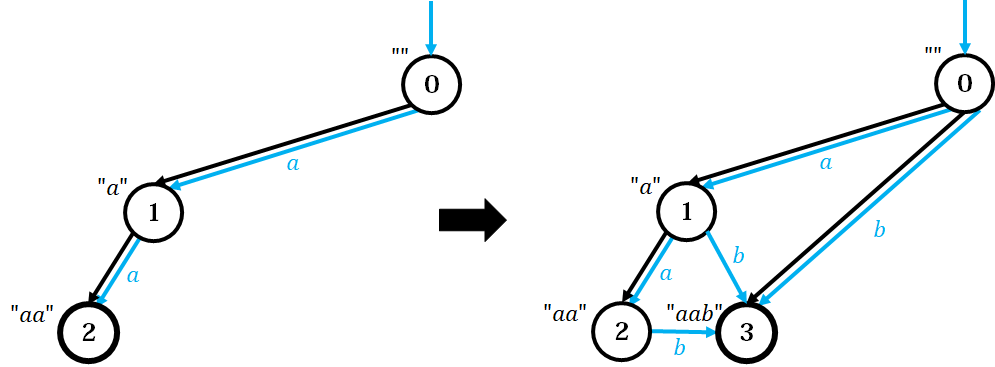
\includegraphics[width=0.9\textwidth]{pic/case1.png}
    \end{figure}
\end{frame}

\begin{frame}{第二种情况}
    \small
    找到了$q$,且len[p]+1==len[q]。这种情况下我们直接令fa[cur]=q然后退出即可。这是因为$p$所对应集合中每个字符串在后面加上一个$ch$都能构成一个$q$对应集合的字符串,而$p$对应集合都是原字符串的后缀,所以$q$对应集合都是新字符串的后缀,应作为$cur$的父亲节点。

    \begin{figure}[H]
        \centering
        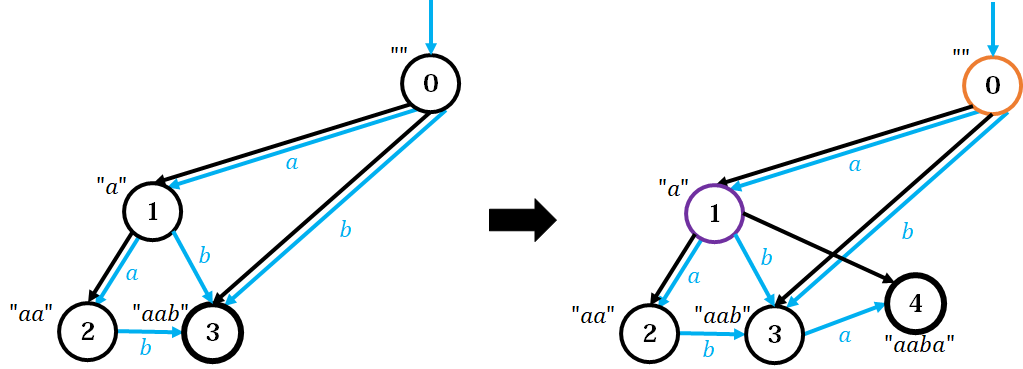
\includegraphics[width=0.9\textwidth]{pic/case2.png}
    \end{figure}
\end{frame}

\begin{frame}{第三种情况}
    \small
    找到了$q$,但len[p]+1$\neq$len[q]。我们新建一个$r$节点,它拥有$q$节点的所有出边,且fa也与$q$节点相同,但是len[r]=len[p]+1。我们从$p$节点继续往上爬,把所有接受$ch$而到达$q$的转移的目标改为$r$(注意只要有一个节点不能接受$ch$那它的祖先都不能接受$ch$,要及时退出循环)。最后令fa[cur]=fa[q]=r。
    
    \begin{figure}[H]
        \centering
        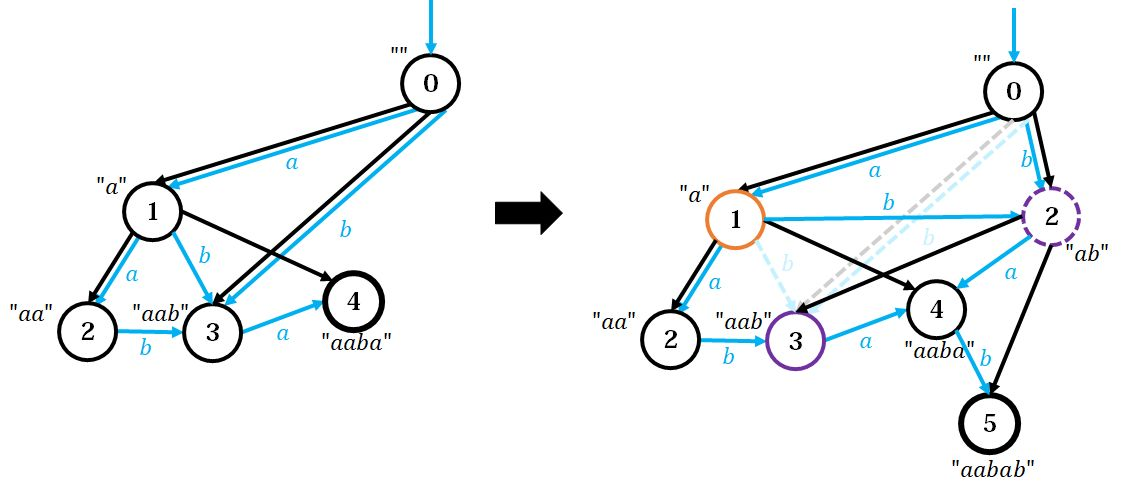
\includegraphics[width=0.8\textwidth]{pic/case3.jpg}
    \end{figure}

    \pause 这里和第二种情况有本质区别,因为$q$不仅仅包含新字符串的后缀,比如下图中3号点除了"ab"还包含了"aab",我们不得不将它拆分开。
\end{frame}

\begin{frame}{一个SAM的例子}
    \small
    下图是字符串"aababb"构成的SAM

    \begin{figure}[H]
        \centering
        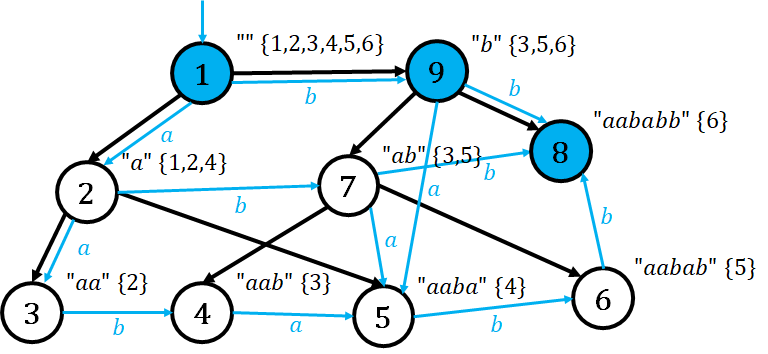
\includegraphics[width=0.8\textwidth]{pic/sameg.png}
    \end{figure}

    复杂度:总状态数不超过$2n-1$,总转移数不超过$3n-4$,构建SAM的复杂度为$O(mn)$,其中$m$为字符集大小。证明见OIwiki
\end{frame}

\begin{frame}{例题选讲}
    \small
    求模式串$P$是不是字符串$S$的子串。

    \pause 【解】建S的SAM,把P放进去跑即可。
\end{frame}

\begin{frame}{例题选讲}
    \small
    求模式串$P$在字符串$S$中的出现次数。

    \pause \vspace{1em}
    【解】建S的SAM,其实就是求$p$对应节点的$endpos$集合的大小,在parent树上dp。

    \pause \vspace{1em}
    对于划分后丢失元素的节点(他所代表的串是$S$的前缀),dp值为子节点dp值之和再加一,其余点则无需加一。其实只要在建SAM的时候让dp[cur]=1即可。

    \pause \vspace{1em}
    小技巧:在parent树上dp的时候不需要dfs,只要把节点按len做一个桶排,然后从大到小枚举,就等价于在parent树上自底向上dp。
\end{frame}

\begin{frame}{例题选讲}
    \small
    求字符串$S$本质不同的子串个数。

    \pause \vspace{1em}
    【解】建S的SAM,从parent树的角度考虑,每个节点代表了len[p]-len[fa[p]]个子串(因为长度不同,自然互不相同)。另外由parent树的划分意义,不同节点代表的子串一定都不同,且任何一个子串必然被parent树上某一点代表。累加该值即可。
\end{frame}

\begin{frame}[fragile]{例题选讲:SPOJ 1811}
    \small
    求字符串$S$与$T$的最长公共子串。

    \pause \vspace{1em}
    【解】建S的SAM,对$T$的每个前缀,求他在$S$中出现过的最长后缀。其实就是把T放进去跑,一直到跑不动了就跳到parent树上的父节点继续跑,跳parent的时候要维护当前最长后缀的长度。

    \pause \vspace{.5em}
    \begin{lstlisting}[language=c++]
    int lcs(char *s)
    {
        int m=strlen(s), l=0, p=1, ans=0;
        for(int i=0;i<m;i++)
        {
            int c=s[i]-'a';
            while(p!=1 && go[p][c]==0)
                p=fa[p], l=len[p]; //维护当前最长后缀长度
            if(go[p][c]) p=go[p][c], l++;
            ans=max(ans,l);
        }
        return ans;
    }
    \end{lstlisting}
\end{frame}

\begin{frame}{例题选讲:(UVA 719) (P1368) 最小表示法}
    \small
    有N组数据,每组给你一串字符串,但是这串字符串是环形的,让你找个位置切开,使得它的字典序最小,输出切开的位置(如果答案不唯一,输出最小位置)

    \pause \vspace{1em}
    【解】遇到循环串的问题一般都先把串复制一遍得到SS,建SS的SAM。

    \pause \vspace{1em}
    SS的SAM能且仅能接受SS的所有子串,所以从根节点出发跑$|S|$步得到的就是$S$的某个循环排列,一直沿最小字典序的转移边跑即可。
\end{frame}

\begin{frame}{例题选讲:UVA 719}
    \small
    给出一个字符串$S$,长度不超过$90000$。询问$q$次,每次给一个$k$,求所有本质不同的子串中,字典序第$k$小的。

    \pause \vspace{1em}
    【解】先建$S$的SAM,求出$size[p]$表示从$p$出发能跑出几个子串,逆拓扑序dp即可。

    \pause \vspace{1em}
    对于一个询问,从根节点出发,每次从小到大枚举字母$ch$,如果$size[go[cur][ch]]\geq k$,就往$ch$走;否则$k=k-size[go[cur][ch]]$,继续枚举$ch$
\end{frame}

\begin{frame}{例题选讲:LNOI2022 串}
    \small
多组数据,每次给定一个英文小写字母构成的字符串 $S$,你需要找到一个尽可能长的字符串序列 $(T_0, T_1, \ldots, T_l)$,满足:

\begin{itemize}
\item $T_0$ 是 $S$ 的子串;
\item $\forall 1 \le i \le l$,$\lvert T_i \rvert - \lvert T_{i - 1} \rvert = 1$;
\item $\forall 1 \le i \le l$,存在 $S$ 的一个长度为 $\lvert T_i \rvert + 1$ 的子串 $S'_i$,使得 $S'_i$ 的长度为 $\lvert T_{i - 1} \rvert$ 的前缀为 $T_{i - 1}$,长度为 $\lvert T_i \rvert$ 的后缀为 $T_i$。
\end{itemize}

输出这样的字符串序列的长度的最大值(即 $l$ 的最大值)。

\vspace{1em}

设 $\sum |S|$ 表示测试点中所有测试数据的字符串长度和。对于 $100 \%$ 的测试数据,$1 \le \lvert S \rvert \le 5 \times {10}^5$,$1 \le \sum \lvert S \rvert \le 1.5 \times {10}^6$。

\end{frame}

\begin{frame}{例题选讲:LNOI2022 串}
    \small
    【题解】观察条件:
    \begin{itemize}
        \item $T_0$ 是 $S$ 的子串;
        \item $\forall 1 \le i \le l$,$\lvert T_i \rvert - \lvert T_{i - 1} \rvert = 1$;
        \item $\forall 1 \le i \le l$,存在 $S$ 的一个长度为 $\lvert T_i \rvert + 1$ 的子串 $S'_i$,使得 $S'_i$ 的长度为 $\lvert T_{i - 1} \rvert$ 的前缀为 $T_{i - 1}$,长度为 $\lvert T_i \rvert$ 的后缀为 $T_i$。
    \end{itemize}

    用$[i,j]$表示子串$S[i...j]$,我们构造一个序列$[i,j]\to [i-1,j-2]\to [i-2,j-4]...$,一直这样下去直到长度为$0$或到头了,得到一列子串,把它倒过来,就符合上面的条件。所以答案显然至少为$\left\lfloor\frac{n}{2}\right\rfloor$。

    \pause \vspace{1em}
    现在考虑正向过程。我们从$T_0=\varnothing$开始,每次左端点往右移一个,同时长度加一。如果想要答案更大,一定要有一个左端点回跳的过程。如果现在位于$[l_2,r_2]$,前面恰好有一个$[l_1,r_1]$和$[l_2,r_2]$是一样的,就可以跳回前面。
\end{frame}

\begin{frame}{例题选讲:LNOI2022 串}
    \small
    枚举最后一次回跳。那么我们现在的过程就是,挑选某一个出现至少两次的子串,设位置分别为$[l_1,r_1]$和$[l_2,r_2]$,从空集开始构造到$[l_2,r_2]$,然后回跳到$[l_1,r_1]$,接下来一直向右构造到底。答案就是
    \begin{equation*}
        r_1-l_1+1+\left\lfloor\frac{n-r_1}{2}\right\rfloor
    \end{equation*}

    \pause \vspace{1em}
    还有一个问题:怎么确保能从空串一直构造到$[l_2,r_2]$?

    \pause \vspace{1em}
    可以从$[l_2,r_2]$开始,向左反向构造,到了$[l_1,r_1]$内就跳回到$[l_2,r_2]$中,再继续向左反向构造。

    \pause \vspace{1em}
    需要SAM。对于一个节点(一个$endpos$等价类),你需要知道他表示的最长串出现了多少次(这需要自底向上dp累加)、第一个$endpos$(这需要自底向上dp取min)、这个等价类中最长的串长(也就是len),然后按上式算答案取最大值即可。
\end{frame}

\section{后缀数组}

\section{参考文献}

\begin{frame}[allowframebreaks]
    \bibliography{ref}
    \bibliographystyle{ieeetr}
    \nocite{*} % used here because no citation happens in slides
    % if there are too many try use:
    % \tiny\bibliographystyle{alpha}
\end{frame}


\begin{frame}
    \begin{center}
        {\Huge\calligra Thank You}
    \end{center}
\end{frame}

\end{document}